\documentclass[journal]{IEEEtran}

%%%%%%%%%%%%%%%%%%%%%%%%%%%%%%%%%

%Linguagem e acentuação\textsl{}
\usepackage[utf8]{inputenc}
\usepackage[T1]{fontenc}
\usepackage{lmodern}

%Imagens
\usepackage{graphicx}

%Tabelas
\usepackage{multicol}
\usepackage{booktabs}
\usepackage{multirow}

%Algoritmo
\usepackage[english, ruled, lined, linesnumbered]{algorithm2e}
\SetKwInOut{Input}{Input}
\SetKwInOut{Output}{Output}


%Gramática
\usepackage[nounderscore]{syntax}
\usepackage{amsmath}
\grammarindent 80pt

%Renomear TABLE para TABELA
%\renewcommand{\tablename}{TABELA.}
%\renewcommand{\refname}{Referências}
%%%%%%%%%%%%%%%%%%%%%%%%%%%%%%%%%

% correct bad hyphenation here
\hyphenation{cons-ta-tar}


\begin{document}
	%
	% paper title
	% can use linebreaks \\ within to get better formatting as desired
	
	\title{A grammatical evolution approach to generate clustering algorithms}
	
	
	\author{
		Vidal D. da Fontoura,
		Ricardo H. R. de Lima
	}
	
	% The paper headers
	%\markboth{Journal of \LaTeX\ Class Files,~Vol.~6, No.~1, January~2007}%
	%{Shell \MakeLowercase{\textit{et al.}}: Bare Demo of IEEEtran.cls for Journals}
	
	% make the title area
	\maketitle
	
	\begin{abstract}
		Nowadays, there is an increase of data generated everywhere and is becoming crucial to analyze and extract the hidden information. Clustering methods, one of the tools to better interpret data, are used for distribution of similar data into groups. Each group has objects that are close to each other considering its characteristics, and different from objects from other groups. Clustering algorithms depends on many parameters that are domain dependent hindering their application. In this context, the field of hyper-heuristics raises as an alternative by allowing the generation of a custom algorithm. In this sense, this work proposes the automatic design of clustering algorithms by using a hyper-heuristic based on Grammatical Evolution (GE). Grammatical Evolution is a type of Genetic Programming that use a Backus-Naur Form Grammar to evolve a population of computer programs to solve a problem. The clustering algorithms are generated for different bases from the UCI repository. The resulting clustering algorithms were compared to the K-means algorithm. The comparison shows promising results. 
		
		
	\end{abstract}
	
	\begin{IEEEkeywords}
		Clustering, Grammatical Evolution, Genetic Programming, Hyper-Heuristic.
	\end{IEEEkeywords}
	
	\IEEEpeerreviewmaketitle
	
	
	\section{Introduction}
	
	More data has been gathered because of modern methods of data collection. The demand for grouping and filtering important data and extract useful information has increased \cite{ahalya2015data}. Clustering is the unsupervised classification of patterns (observations, data items, or feature vectors) into groups (clusters) \cite{jain1988algorithms}. Clustering approaches applications have increased in various areas of Artificial Intelligence, data mining, image recognition, data statistics, etc. The main goal is to determine the intrinsic grouping in a set of unlabeled data \cite{ahalya2015data}.
	
	The main problem in the application of clustering methods is that the algorithms depends on many parameters that are domain dependent hindering their application. In this context, the field of hyper-heuristics raises as an alternative by allowing the generation of a custom algorithm. Hyper-heuristics is a field of study which aims to be able to automatically create novel algorithms designed to perform better on certain classes of problem than would a general algorithm modified by hand for that purpose \cite{harris2015comparison}. The automatic design of the algorithms using Hyper-heuristics are often done through the use of genetic programming techniques. Genetic Programming (GP) is a type of Evolutionary Algorithm (EA) that has gained more interest over the years. GP is a domain-independent method that genetically breeds a population of computer programs to solve a problem, it evolves the solutions by the application of selection, mutation and crossover operators \cite{poli2014genetic}. The GP provides a way to automate one of the most expensive and time-consuming aspects of the software engineering process: the production of the code itself \cite{langdon2013optimising}. The GP algorithms are responsible for select individual parts (functions, routines, pieces of code) to build an algorithm and then evaluate it in order to search for a design that best solve a certain type of problem.
	
	Deeper in the idea of evolving computer programs, one of the used approaches in Genetic Programming, is the Grammatical Evolution (GE), where a BNF (Backus-Naur Form) grammar is used to generate sentences for a given language, this sentences are mapped into the computer programs that are evaluated by the algorithm. Finally, the generated algorithm is executed and its performance is used as feedback for the evolutionary process.
	
	Based on the presented topics, this paper proposes the automatic design of clustering algorithms by applying the Grammatical Evolution approach. In order to guide this work we defined the research question for this study:
	
	\begin{itemize}
		\item Q1: Is it possible to generate good clustering algorithms.
	\end{itemize}
	
	To answer this question, the following approach is adopted: the clustering algorithms are generated for different bases from the UCI repository. The resulting clustering algorithms are  compared to the K-means algorithm. 
	
	This paper is organized as follows. In Section \ref{sec:theoretical_foudation}, has a description about the topics that are important for the full understanding of the paper. In Section \ref{sec:methodology} is described how was the design of the method for generation of clustering algorithms using GE. The Section \ref{sec:experiments} presents the experiments that were ran, the results obtained, and the comparison with the K-means algorithm. In the Section \ref{sec:discussion} a discussion about the proposed research questions is presented. Section \ref{sec:threats} presents some threats to validity . Finally, the Section \ref{sec:conclusion} presents the conclusion.
	
	
	\section{Theoretical Foundation} \label{sec:theoretical_foudation}
	
	This section reviews important concepts used in this paper. First, genetic programming is presented. Then, grammatical evolution is addressed, i.e., how the grammar supports the generation of programs, and how to choose and map the individuals into programs. Moreover, the clustering problem is described.
	
	
	\subsection{Genetic Programming}
	
	Genetic Programming (GP) is a systematic method for getting computers to automatically solve a problem from a high-level statement of what need to be done \cite{koza2005genetic}. Having a similar behavior to Genetic Algorithms (GAs), GP iteratively evolves a population of computer programs, applying the selection, crossover and mutation operators, in order to improve their fitness, and increase the chances of an individual being part of future generations.
	
	Different from the AG, the GP works with computer programs, and because of this, the use of a different structure for individual's representation is needed. There are many ways to represent individuals, some of the most used are: the syntax tree and linear representation.
	
	The original formulation of genetic programming was done with a tree representation. Here, each node on the tree is a function which takes its children as inputs and sends its output to its parent. Each sub-tree is a complete sub-program. However, there is no capacity for parts of the tree to be reused in a calculation (like in loops), which make some things more difficult to be done \cite{harris2015comparison}. 
	
	Grammatical evolution, a genetic programming variant, uses a genotype that represents a set of nodes, which are translated to a list of grammatical expansions which eventually produce its nodes. This potentially allows the user to have a lot more control over the search space, and also facilitates the use of multiple data types in the algorithm. The genotype is represented linearly but can be decoded into a tree for execution and evaluation. In terms of what can be represented, unless restricted in its grammar, this GP variant has the same power over the search space as tree GP \cite{harris2015comparison}.
	
	
	\subsection{Grammatical Evolution} \label{subsection:grammaticalEvolution}
	
	Grammatical evolution is a grammar based form of genetic programming. GE accomplishes the mapping process by combining a context free grammar (CFG) with a rule selection mechanism implemented using a genetic algorithm \cite{byrne2015optimising}.
	
	The main difference between GE and GP, is that in GP, both genotype and phenotype of the individual that is under evolution are derivation trees, whilst in GE, genotype and phenotype have different encoding structures. The genotype is represented as a linear string of codons (sequence of 8 bits) of variable size, which is then decoded into a vector of integers. The phenotype, which is the structure that defines fitness, is represented by a derivation tree (resulting from the application of a grammar) \cite{cerri2013grammatical}. The clear distinction between the genotype and phenotype in GE allows the evolutionary process to be performed on the search space (variable length linear genotypic) without needing to tailor the diversity-generating operator to the nature of the phenotype \cite{sabar2013grammatical}.
	
	The grammar is a set of structural rules that define the composition of sentences for a given language. Grammatical rules provide a concise way of restricting a language while allowing endless variation through recursive application of the rules\cite{byrne2015optimising}. The grammar is represented by Backus-Naur Form (BNF). The program is generated using an integer vector, where each codon (vector position) value, is used to determine which production rule in the BNF grammar will be used.
	
	\begin{figure}[!htb]
		\centering
		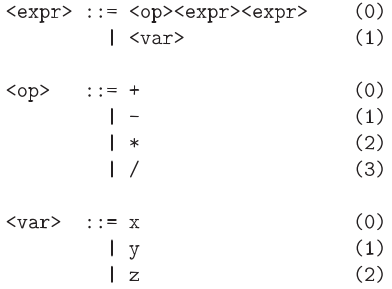
\includegraphics[scale=.6]{figures/grammar.png}
		\caption{Example of basic grammar. \cite{ryan1998grammatical}}
		\label{fig:grammar}
	\end{figure}
	
	The Figure \ref{fig:grammar} shows a basic BNF (Backus-Naur Form) grammar, that can be used to generate simple math equations. In the group of terminal nodes, we have: +, -, *, /, as operations and x, y and z as variables. For the non-terminal nodes, we have: $<$op$>$, $<$expr$>$ and $<$var$>$.
	
	\begin{figure}[!htb]
		\centering
		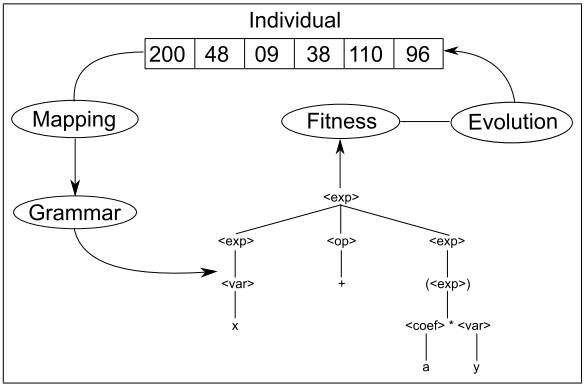
\includegraphics[scale=.4]{figures/ge_algo.png}
		\caption{Basic scheme for mapping process. \cite{cerri2013grammatical}}
		\label{fig:ge_algo}
	\end{figure}
	
	A mapping process is needed to convert the bit string (genotype) into the derivation tree (phenotype), so the fitness can be evaluated. The mapping process is shown in Figure \ref{fig:ge_algo}. Starting from the bit string or integer vector, each codon has its value used in the Equation \ref{eq:map} to select a derivation rule from the grammar:
	
	\begin{equation}\label{eq:map}
	GR_i = int~~mod~~nr_i
	\end{equation}
	
	where $GR_i$ is the index of the grammar rule to be selected in non-terminal $i$, $int$ is the codon integer value and $nr_i$ is the number of rules available for derivation in non-terminal $i$. The operator $mod$ returns the remainder of the division between two numbers.
	
	
	\subsection{Clustering}
	
	The Clustering problem consists in partitioning a dataset into subgroups such that items belonging to the same group are more similar than those belonging to different groups \cite{boric2007genetic} \cite{ahalya2015data}. The clustering approaches application has widely increased in the areas of Artificial Intelligence, pattern recognition, image processing, medicine, marketing, data mining, compression of images or data, statistics, etc. \cite{ahalya2015data}.
	
	The most widely used and studied clustering algorithm is \textit{K-means}. Given a set of $n$ data objects in a Real $n$-dimensional space, $R^n$, and an integer $k$, the problem is to determine a set of $k$ objects in $R^n$, called \textit{centers}, so as to minimize the mean squared distance from each data object to its nearest center \cite{kanungo2002efficient}.
	
	
	\subsubsection{Silhouette Index}
	\label{sec:sillhouetteIndex}
	
	There are many algorithms for partitioning a set of objects into $k$ clusters, such as the $k$-means method \cite{kanungo2002efficient}. Since similarity is fundamental to the definition of a cluster, a measure between two items is essential to most clustering techniques. Because of the variety of feature types and scales, the distance measure (or measures) must be chosen carefully. It is most common to calculate the \textit{dissimilarity} between two items. One of the most popular metric for continuous features is the \textit{Euclidean distance} \cite{jain1988algorithms}.
	
	The Silhouettes are useful when the proximities are on a ratio scale (as in the case of Euclidean distances). For the construction only two things are necessary: the groups obtained by some clustering technique, and the collection of all proximities between objects. For each object $i$ there is a value called $s(i)$, that can be defined in term of two functions, here defined in terms of dissimilarity. For any item $i$ part of a cluster A, when cluster A contains other objects apart from $i$, we can compute:
	
	\begin{equation} \label{eq:a_i}
	a(i) = average~dissimilarity~of~i~to~all~other~objects~of~A
	\end{equation}
	
	In \ref{fig:silhouette}, this is the average length of all lines within A. Now, considering any cluster C which is different from A, for the object $i$, we can compute:
	
	\begin{equation} \label{eq:d_i}
	d(i, C) = average~dissimilarity~of~i~to~all~objects~of~C
	\end{equation}
	
	In \ref{fig:silhouette}, this is the average length of all lines going from $i$ to C. Then, after computing $d(i, C)$ for all $C \neq A$, the smallest value is selected as denoted the function \ref{eq:b_i}.
	
	\begin{equation} \label{eq:b_i}
	b(i) = minimun~d(i, C)~for~all~C \neq A
	\end{equation}
	
	\begin{figure}[!htb]
		\centering
		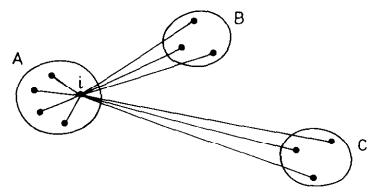
\includegraphics[scale=.6]{figures/silhouette_img.png}
		\caption{Illustration of the elements involved in the computation of the silhouette. \cite{rousseeuw1987silhouettes}}
		\label{fig:silhouette}
	\end{figure}
	
	The function $b(i)$ is used to define the cluster neighbor of item $i$. This is likely the second best choice for object $i$. The function $b(i)$ depends on the availability of other clusters apart from $A$, so we have to assume that the number os clusters is greater than one.
	
	Finally, the value of $s(i)$ is obtained by combining $a(i)$ and $b(i)$, as in the Equation \ref{eq:s_i}:
	
	\begin{equation} \label{eq:s_i}
	s(i) = \frac{b(i) - a(i)}{max\{a(i), b(i)\}}
	\end{equation}
	
	When cluster $A$ contains only a single object it is unclear how $a(i)$ should be defined, and then in this case the value of $s(i)$ is set to zero. This choice is taken because
	\begin{center}
		$-1 \le s(i) \le 1$
	\end{center}
	
	for each object $i$, and zero is the most neutral value. When $i$ is closer to 1, it implies that the object $i$ is "well-clustered", because the dissimilarity $a(i)$ is much smaller than the smallest "between" dissimilarity $b(i)$. On the other hand, when $i$ is closer to -1, it implies that $i$ has been "missclassified", because $a(i)$ is much larger than $b(i)$, and $i$ is closer to $B$ than $A$.
	
	In summary, $s(i)$ measures how well object $i$ matches the clustering at hand, in other words, how well the item $i$ has been classified.
	
	
	\section{Methodology} \label{sec:methodology}
	
	Our proposed method consists on applying GE to generate clustering algorithms. A specific grammar was designed  using  Backus-Naur form. The grammar is shown below:
	
	\begin{grammar}
		<GE> ::= <initialization> <distance> <command> 
		\\ <initialization> ::= "random" <k> | "uniform" <k>
		\\ <command> ::= <movement> | <movement> <command>
		\\ <movement> ::= "joinClusters" | "splitClusters" | "moveAverage" | "moveBetween" | "moveNear" 
		\\ <k> ::= "4" | "6" | "8" | "10" | "0"
		\\ <distance> ::= "eucledian" | "manhattan" | "chebyshev"
		\label{ge-clustering-grammar}
	\end{grammar}
	
	The first line specifies the main algorithm components: initialization, distance and command. 
	
	For the initialization node two possibilities of terminal nodes were implemented: random and uniform. The random initialization consists of randomly select objects as centroids of the clusters. The uniform initialization consists on finding the minimum and maximum values for each attribute of the dataset. Then, this information is used to uniformly select the coordinates (within this range) for centroids. Moreover, for both initialization methods, an initial value of $k$ (number of clusters) is chosen between five possible values: 4, 6, 8, 10 and 0. If the chosen $k$ value is equals to 0 it will be drawn a random number between 2 and 5. Note that, this $k$ value is an initial value because the grammar allows to create or destroy clusters. 
	
	In the case of the distance component, three possibilities of distance functions were implemented: \textit{Euclidean}, \textit{Manhattan} and \textit{Chebyshev}. The selected distance function will be used in all other functions that requires information of distance between the data.
	
	The command component is the main body of the structure and it allows the creation or destruction of clusters as well as movements of data from one cluster to another. This component can potentially generate infinite programs since it has a recursion. In order to avoid the generation of infinite programs, a maximum depth value was setup to 400. The  terminal node are described at next.
	
	\begin{itemize}
		\item JoinClusters: this terminal selects one random cluster, then computes the nearest cluster and merge both.
		\item SplitClusters: this terminal searches for the cluster which has the highest average distance between the objects and its centroid and splits it. 
		\item MoveAverage:  this terminal gets one random object and calculates for each cluster the distance to all objects. The cluster whose average distance is the lowest will receive the selected object.
		\item MoveBetween: the terminal selects one random cluster and computes the nearest cluster. Then gets the object from the second cluster which has the lowest distance to the first centroid cluster and moves it.
		\item MoveNear:  the terminal gets one random object and calculates the distance to all clusters centroids. The cluster whose distance is the lowest between the centroid and the selected object will receive it.
	\end{itemize}
	
	The designed grammar can generate clustering algorithms based on an integer vector as described on subsection \ref{subsection:grammaticalEvolution}. As sampled below, this process is illustrated by beginning with the integer vector (genotype) and then follows the steps to decode it into a clustering algorithm (phenotype). Lets assume the following integer vector:
	
	[199, 45, 172, 156, 157, 137, 191, 56, 27, 103, 5, 109, 81, 160, 124, 5, 182, 121, 247, 68, 180, 182, 100, 143, 141, 109]
	
	The first gene is 199 and it is the entry object. The \textit{initialization} is the first non-terminal node. The next position in the vector is 45 and we have 2 options (\textit{random} and \textit{uniform}); thus 45 mod 2 will result in 1 which selects \textbf{uniform}. The initialization requires another value for the initial $k$ value. Following the vector, the next value is 172; There are 5 possibilities for k. Hence 172 mod 5 = 2, which is the index of the value \textbf{8}. The \textit{initialization} is ended. The second non-terminal node is \textit{distance}. There are three possible terminal nodes options. Next value on the vector is 156. The mod between 156 and 3 results in 0 which indicates to select \textbf{Euclidean}. Now ,it is necessary to decode the \textit{command} non-terminal node. Next position is 157 and two possibilities (\textit{movement} or \textit{movement + command}). Then 157 mod 2 = 1. Therefore, the selected one is \textbf{movement + command}. First we need to decode \textbf{movement} and the next step will be decoding the \textbf{command}. Next position is 137 and there are 5 possibilities, thus the result is 2. The index 2 in the grammar is the \textbf{moveAverage} option. Now we have to evaluate the \textbf{command}; as before, we have 2 choices. As 191 mod 2 = 1, \textbf{movement + command} is selected again. This is repeated until the mod results in 0 and then last \textbf{movement} is selected or until the max depth limit (400) is exceeded. The entire decoded clustering algorithm is present in Algorithm \ref{clustering-algoritm-example}
	
	\begin{algorithm}[!htb]
		\label{clustering-algoritm-example}
		Initialization initialization = new UniformInitialization(); \\
		DistanceFunction distanceFunction = new EucledianFunction(); \\
		int initialK = 8; \\
		boolean finished = false; \\
		int evaluations = 1000;\\
		ClusteringState 
		clusteringState = initialization.createInitialClusters(initialK); \\
		\While{!finished}{
			moveAverage(clusteringState); \\
			splitClusters(clusteringState); \\
			moveBetween(clusteringState); \\
			moveNear(clusteringState); \\
			joinClusters(clusteringState); \\
			joinClusters(clusteringState);\\
			
			finished = $!clusteringState.changed()$   $|| $		$evaluations>maxEvaluations$}{
			
		}
		\caption{Pseudo code from a decoded algorithm}
	\end{algorithm}
	
	The pseudo-code presented in algorithm \ref{clustering-algoritm-example} is an example of the algorithms generated by the grammar. The stopping criterion in the generated algorithms is fixed using two conditions: first, if no changes occurs to the clustering state or if the maximum number of evaluations is exceeded. This can be seen at line 14 of the pseudo-code. The maximum number of evaluations was adjusted to 1000 after some experiments.
	
	The next step is the grammatical evolution process which consists of evolving populations of integer vectors through a genetic algorithm (GA). The individuals are converted to clustering algorithms and then applied to a cluster dataset. To evaluate the individuals a fitness function was designed as shown on Equation \ref{equation:fitness}.
	
	\begin{equation} \label{equation:fitness}
		fitness = \frac{\sum_{i=1}^e \frac{\sum_{j=1}^{p} s_{ij}}{p}}{e}
	\end{equation}
	
	The $e$ value represents the number of independent executions of the clustering algorithm, it was fixed to 10. The $p$ value is the number of objects of the respective dataset being used. The $s_{ij}$ is the silhouette index (explained in sub-section \ref{sec:sillhouetteIndex}) of the $j^{\text{th}}$ object of the $i^{\text{th}}$ execution. Basically the fitness function is given by the average of the silhouette value for every object of the dataset in each execution of the clustering algorithm.
	
	The GA used to evolve the clustering algorithms is similar to a traditional GA, however the individual solutions have not fixed length, whereas the generated algorithms can have different sizes. Since the solutions doesn't have a fixed length, it is possible by the application of a crossover or mutation that one individual has less genes than the required for building a clustering algorithm. The approach for this situation is to continue getting the integer values from the beginning of the individual in order to fill all functions required by a clustering algorithm. Also, it is possible to occur the inverse situation: when an individual is bigger than the necessary to build a clustering algorithm. The strategy adopted here is to simply discard the portion that is not being used. It is worthwhile to mention that individuals in GE do not necessarily use all their genes to be decoded to a program. A prune operator was proposed by \cite{ryan1998grammatical} to reduce the possibilities of crossover operations being applied on genes that are not decoded to a program. The prune operator consists on a given probability, truncate the offspring generated by the crossover and mutation operators. Another operator that was proposed to deal with GE is the duplication operator inspired by the biological background. It consists on duplicating a random number of genes to the end of the original individual, also given a probability of occurrence. The main idea here is to duplicate the genes in order to increase their presence on the overall individual.
	
	
	\section{Experiments} \label{sec:experiments}
	
	The proposed GA in this work was implemented using the open source architecture from JMetal framework \cite{jMetal} because its easy to extend, and also has a well organized structure and active community.  
	
	A set of experiments were conducted using  four well-known clustering dataset from UCI machine learning database \cite{uci}. The Table \ref{uci-experiments} shows the amount of instances, numbers of attributes and the data type of the datasets. 
	
	The GE was executed 10 independent runs with each dataset using the same configuration presented in table \ref{ga-configuration}. The evaluation of the individuals was made using the fitness function presented on equation \ref{equation:fitness}.
	
	The results were summarized by means of average, standard deviation, minimum and maximum values of the fitness value, from the best individual of each run of the GA. The amount of clusters ($k$) found are also presented.
	
	In order to make comparisons, the K-means algorithm was executed 10 times with different $k$ values. The $k$ value for K-means was varied within the range 2 to 7 and only the best $k$ configuration (the one that obtained the highest fitness values) is presented. 
	
	\begin{table}[]
		\centering
		\caption{Configuration used in the GA}
		\label{ga-configuration}
		\begin{tabular}{|l|l|}
			\hline
			\textbf{Crossover  |  Probability}         & Single Point  | 0.95     \\ \hline
			\textbf{Mutation | Probability}            & Integer Mutation          |  0.10 \\ \hline
			\textbf{Prune  | Probability}      & Prune Operator           | 0.05   \\ \hline
			\textbf{Duplication Operator | Probability} & Duplication   | 0.05     \\ \hline
			\textbf{Population}                        & 100                               \\ \hline
			\textbf{Generations}                       & 200                               \\ \hline
		\end{tabular}
	\end{table}
	
	\begin{table}[]
		\centering
		\caption{UCI datasets used in the experiments}
		\label{uci-experiments}
		\begin{tabular}{|l|l|l|l|l}
			\cline{1-4}
			\textbf{Dataset Name}                                           & \multicolumn{1}{l|}{\textbf{Intances}} & \multicolumn{1}{l|}{\textbf{Attributes}} & \textbf{Type}     \\ \hline
			\begin{tabular}[c]{@{}l@{}}Pima Indians\\ Diabetes\end{tabular} & 768                                    & 8                                        & Integer, Real     \\ \hline
			Stalog (Hearth)                                                 & 270                                    & 13                                       & Categorical, Real \\ \hline
			Iris                                                            & 150                                    & 4                                        & Real              \\ \hline
			\begin{tabular}[c]{@{}l@{}}Glass\\ Identification\end{tabular}  & 214                                    & 10                                       & Real              \\ \hline
		\end{tabular}
	\end{table}
	
	Table \ref{results-ga-and-kmeans} shows the results described above. 
	
	\begin{table*}[]
		\centering
		\caption{Results of GA best individual and also the fitness obtained by K-means algorithm}
		\label{results-ga-and-kmeans}
		\begin{tabular}{|c|c|c|c|c|c|}
			\hline
			\textbf{Dataset}           & \textbf{Algorithm} & \textbf{Statistics} & \textbf{Fitness} & \textbf{k}    & \textbf{Kruskal-Wallis Test}   \\ \hline
			\multirow{8}{*}{Pima Indians Diabetes} & \multirow{4}{*}{GA}           & Average                        & \textbf{0.605378}                    & 2                        & \multirow{8}{*}{TRUE} \\ \cline{3-5}
			&                               & Std Dev                        & 0.009389                    & 0                        &                       \\ \cline{3-5}
			&                               & Min                            & 0.586249                    & 2                        &                       \\ \cline{3-5}
			&                               & Max                            & 0.6168851                   & 0                        &                       \\ \cline{2-5}
			& \multirow{4}{*}{K-Means}      & Average                        & 0.5701015                   & \multirow{4}{*}{Fixed 2} &                       \\ \cline{3-4}
			&                               & Std Dev                        & 0.0000000                   &                          &                       \\ \cline{3-4}
			&                               & Min                            & 0.5701015                   &                          &                       \\ \cline{3-4}
			&                               & Max                            & 0.5701015                   &                          &                       \\ \hline
			\multirow{8}{*}{Statlog (Heart)}       & \multirow{4}{*}{GA}           & Average                        & \textbf{0.410924}                    & 2                        & \multirow{8}{*}{TRUE} \\ \cline{3-5}
			&                               & Std Dev                        & 0.019960                    & 0                        &                       \\ \cline{3-5}
			&                               & Min                            & 0.381797                    & 2                        &                       \\ \cline{3-5}
			&                               & Max                            & 0.44972                     & 2                        &                       \\ \cline{2-5}
			& \multirow{4}{*}{K-Means}      & Average                        & 0.383325                    & \multirow{4}{*}{Fixed 2} &                       \\ \cline{3-4}
			&                               & Std Dev                        & 0.001523                    &                          &                       \\ \cline{3-4}
			&                               & Min                            & 0.382144                    &                          &                       \\ \cline{3-4}
			&                               & Max                            & 0.385095                    &                          &                       \\ \hline
			\multirow{8}{*}{Glass Identification}  & \multirow{4}{*}{GA}           & Average                        & 0.602340                    & 2                        & \multirow{8}{*}{TRUE} \\ \cline{3-5}
			&                               & Std Dev                        & 0.005321                    & 0                        &                       \\ \cline{3-5}
			&                               & Min                            & 0.593869                    & 2                        &                       \\ \cline{3-5}
			&                               & Max                            & 0.610906                    & 2                        &                       \\ \cline{2-5}
			& \multirow{4}{*}{K-Means}      & Average                        & \textbf{0.624821}                    & \multirow{4}{*}{Fixed 2} &                       \\ \cline{3-4}
			&                               & Std Dev                        & 0.000007                    &                          &                       \\ \cline{3-4}
			&                               & Min                            & 0.624818                    &                          &                       \\ \cline{3-4}
			&                               & Max                            & 0,624836                    &                          &                       \\ \hline
			\multirow{8}{*}{Iris}                  & \multirow{4}{*}{GA}           & Average                        & 0.6442809                   & 2                        & \multirow{8}{*}{TRUE} \\ \cline{3-5}
			&                               & Std Dev                        & 0.0135472                   & 0                        &                       \\ \cline{3-5}
			&                               & Min                            & 0.6244826                   & 2                        &                       \\ \cline{3-5}
			&                               & Max                            & 0.6679046                   & 2                        &                       \\ \cline{2-5}
			& \multirow{4}{*}{K-Means}      & Average                        & \textbf{0.6813042}                   & \multirow{4}{*}{Fixed 2} &                       \\ \cline{3-4}
			&                               & Std Dev                        & 0,0000000                   &                          &                       \\ \cline{3-4}
			&                               & Min                            & 0,6813042                   &                          &                       \\ \cline{3-4}
			&                               & Max                            & 0,6813043                   &                          &                       \\ \cline{3-4}							 \hline
		\end{tabular}
	\end{table*}
	
	\begin{table*}[]
		\centering
		\caption{Statistic of execution time of the algorithms}
		\label{resultsTimeExecution}
		\begin{tabular}{|c|c|c|c|c|}
			\hline
			\textbf{Dataset}                       & \multicolumn{1}{l|}{\textbf{Statistics}} & \multicolumn{1}{l|}{\textbf{\begin{tabular}[c]{@{}l@{}}GA Execution\\ Time (h)\end{tabular}}} & \multicolumn{1}{l|}{\textbf{\begin{tabular}[c]{@{}l@{}}GA Best Individual \\ Execution Time (ms)\end{tabular}}} & \multicolumn{1}{l|}{\textbf{\begin{tabular}[c]{@{}l@{}}K-Means\\ Execution Time (ms)\end{tabular}}} \\ \hline
			\multirow{4}{*}{Pima Indians Diabetes}       & Average                                  & 261.7                                                  & 10581.7                                                                                                         & 
			102.6                                                                                               \\ \cline{2-5} 
			& Std Dev                                  & 56.5                                                                                       & 922.9                                                                                                           & 39.3                                                                                               \\ \cline{2-5} 
			& Min                                      & 199.0                                                                                         & 8809.9                                                                                                           & 71.0                                                                                                 \\ \cline{2-5} 
			& Max                                      & 349.0                                                                                        & 11933.0                                                                                                          & 71.0                                                                                                \\ \hline
			\multirow{4}{*}{Statlog (Heart)}       & Average                                  & 38.6                                                                                          & 1468.8                                                                                                          & 20.3                                                                                                \\ \cline{2-5} 
			& Std Dev                                  & 11.1                                                                                          & 243.5                                                                                                           & 11.6                                                                                                \\ \cline{2-5} 
			& Min                                      & 23.0                                                                                          & 885.0                                                                                                           & 7.0                                                                                                 \\ \cline{2-5} 
			& Max                                      & 56.0                                                                                          & 1738.0                                                                                                          & 52.0                                                                                                \\ \hline
			\multirow{4}{*}{Glass Identification}  & Average                                  & 19.6                                                                                          & 2602.1                                                                                                          & 14.8                                                                                                \\ \cline{2-5} 
			& Std Dev                                  & 2.1                                                                                           & 502.69                                                                                                          & 13.0                                                                                                \\ \cline{2-5} 
			& Min                                      & 15.0                                                                                          & 1610.0                                                                                                          & 3.0                                                                                                 \\ \cline{2-5} 
			& Max                                      & 22.0                                                                                          & 3185.0                                                                                                          & 45.0                                                                                                \\ \hline
			\multirow{4}{*}{Iris}                  & Average                                  & 8.5                                                                                           & 1074.5                                                                                                          & 15.1                                                                                                \\ \cline{2-5} 
			& Std Dev                                  & 2.7                                                                                           & 383.9                                                                                                           & 14.9                                                                                                \\ \cline{2-5} 
			& Min                                      & 4.5                                                                                           & 558.0                                                                                                           & 7.0                                                                                                 \\ \cline{2-5} 
			& Max                                      & 12.0                                                                                          & 1786.0                                                                                                          & 59.0                                                                                                \\ \hline
		\end{tabular}
	\end{table*}
	
	Looking at table \ref{results-ga-and-kmeans}, it is possible to observe that for the Pima Indian Diabetes database, our approach reached 0.605 average of the fitness values obtained by the bests individuals of 10 executions, while the K-means algorithm obtained a lower value equal to 0.570 on 10 executions.
	
	In the case of the Statlog (Heart) database,  the GA obtained a better average value of 0.410 while K-means algorithm reached 0.383. According to the Kruskal-Wallis statistic test, these results have statistical difference.
	
	In the Glass database, the results of GA have lower values than K-means, 0.603 and 0.624 respectively. Also with statistical difference according to Kruskal-Wallis test. 
	
	Finally, for the Glass database the best individuals of GA obtained 0.644 and the K-means reached 0.681, again with statistic difference according to Kruskal-Wallis test.
	
	Moreover, it is possible to note that for all 10 executions of the GA, the generated algorithms used two clusters. In the case of the K-means algorithm, the results that presented the highest fitness values were also using $k=2$. For the sake of space the results with $k = (3,4,5,6,7)$ were suppressed.
	
	Table \ref{resultsTimeExecution} presents some computational time information of the algorithms. The statistic summary of 10 GA executions, in hours, is presented in the third column. In the fourth column shows the statistics summary of time taken, in milliseconds, to execute 10 times the best individual found by the GA. The fifth column presents the statistics summary of executing 10 times the K-means algorithm.
	
	
	\section{Discussion} \label{sec:discussion}
	
	After the conducted experiments it was possible to answer the research questions. Based on the experiments conducted is was possible to verify that the generated algorithms are able to reach good and acceptable values for the  fitness function (which is based on the silhouette index). The fitness values obtained by the generated algorithms in two of four experiments were higher than the ones obtained by the K-means algorithm. The difference between the fitness values obtained by K-means and the approach proposed here is very small. Our conclusion was that, in this context the generated algorithms proved to be competitive to K-means algorithm. It is possible to highlight, one advantage of the proposed approach: there is no need to configure the $k$ value which usually is a non-trivial task as mentioned by many authors \cite{pham2005selection, yan2005methods, tibshirani2001estimating}.
	
	
	\section{Threats to validity} \label{sec:threats}
	
	Some threats to validity are discussed in this section:
	
	\begin{itemize}
		\item The parameter's configuration was not tuned due to time constraints. The configuration was selected mainly based on literature works and some empirical experiments. It is possible that using a tuned configuration the results get improvements.
		\item The experiments were conducted using only 4 datasets: It is necessary to execute more experiments with a broader range of datasets in order to evaluate if the same behavior is maintained.
		\item The results strongly depends on the used grammar and future works include new rules.
	\end{itemize}
	
	
	\section{Related Work} \label{sec:related_work}
	
	In \cite{lourencco2012evolving} they proposed a Grammatical Evolution framework to the automatic design of Evolutionary Algorithms. The grammar defined has the ability to combine components that regularly appear in existing evolutionary algorithms, aiming to achieve novel and fully functional optimization methods. They used the Royal Road Functions to verify the capacity of the framework to evolve algorithms. The results obtained show that the framework is able to evolve simple evolutionary algorithms that can effectively solve the Royal Road instances. In some cases, unusual design solutions provided by the framework show competitive results with standard approaches.
	
	The work of \cite{miranda2015gefpso} was one of the papers used as base for this research. In the paper they describe the creation of a framework for PSO Optimization using Grammatical Evolution. This paper also describes how to use a grammar to generate the algorithms and evaluate them by using integer vector individuals, and how to define the grammar (the production rules and expressions used). As in this work, they presented a grammar to generate configurations for the PSO algorithm. They performed experiments on the benchmark problems, and demonstrate that the proposed method generates useful designs which achieved competitive solutions when compared to well succeeded algorithms from the literature.
	
	The paper of \cite{burke2012grammatical} show that GP approaches have been employed to automatically design constructive heuristics for solving problems. These algorithms obtained results superior to human-created heuristics, but they do not generally obtained results from the same quality as local search heuristics. So in they research, they proposed the use of Grammatical Evolution to automatically generate good quality local search algorithms, that maintain their performance on new problem instances.
		
	The paper of \cite{bolton2015optimizing} is about the challenging task that is to design efficient algorithms for difficult combinatorial optimization problems. There is a variety of heuristic, meta-heuristic and hyper-heuristic methods, showing in some cases that combining algorithms can produce better results than individual performance. In the paper they propose the use of Genetic Programming to automate the design of algorithms to put into practice against the Clustering problem. They created some functions that represents common operations made in clustering algorithms to represent the nodes required by GP, so the evolutionary could produce algorithms based on these functions and then evaluate its fitness based on how well the new algorithm classify data.
		
	All the works mentioned have applications of GP for automatically design algorithms for solving problems. The paper of \cite{lourencco2012evolving} uses GE to evolves evolutionary algorithms for optimizing the Royal Road Functions, the grammar used was created by using the common functions present in standard GA, like population size, selection, mutation, crossover, replacement, its parameters, etc. The work of \cite{miranda2015gefpso} proposes the use of GE for finding good configurations for the PSO algorithm. The grammar was defined with the main parameters of the PSO, like population size, velocity calculation, update-velocity method, global best method, etc. But they made experiments only in the mono-objective version of the algorithm. The paper of \cite{burke2012grammatical} say that GP approaches can obtain better results than human-created heuristics, but equally results when it comes to local search methods to prove that automatic designed algorithms can maintain the good performance over different problem instances. Finally the paper of \cite{bolton2015optimizing} presented the idea of using GP for the Clustering problem, using common operation for moving and classify objects as functions for built the algorithms. There is other approaches for the Clustering problem using GP like the paper of \cite{boric2007genetic}, that uses Information Theoretic Fitness Measure -- a probabilistic interpretation of the space of objects -- for classifying data.
	
		
	\section{Conclusion} \label{sec:conclusion}
	
	Grammatical evolution is a form of genetic programming which uses a grammar to map the genotype into the phenotype. The definition of a good rules set is crucial for the success of an GE approach. This work presented the use of GP and design of a BNF grammar in order to evolve a population of clustering algorithms through a GA. To evaluate the generated algorithms: a fitness function based on the silhouette index was implemented.
	
	A set of experiments were conducted and compared with the K-means algorithm using UCI databases. In 2 of 4 datasets the proposed approach reached higher values when compared with the K-means algorithm.
	
	Based on the conducted experiments, it is possible to conclude that the proposed approach can generated good clustering algorithms.
	
	%Referências
	\bibliographystyle{plain}
	\bibliography{references}
	
	% that's all folks
\end{document}